\documentclass[a4paper,12pt,twoside, openany]{book}

\usepackage[a4paper,left=1.25in,right=1in,top=0.75in, bottom=0.75in]{geometry}
\usepackage{color}
\usepackage{courier}

\usepackage{caption}
\captionsetup{labelfont=bf}
\usepackage{subcaption} 

\usepackage{tgpagella} % text only
\usepackage{mathpazo}  % math & text

\usepackage{enumitem}

\usepackage{array}
\newcolumntype{P}[1]{>{\centering\arraybackslash}p{#1}}
\newcolumntype{M}[1]{>{\centering\arraybackslash}m{#1}}

\usepackage{hyperref}
\hypersetup{
    colorlinks = true,
    linkcolor=blue,
    %anchorcolor [black]
    %citecolor [green]
    %filecolor [cyan]
    %menucolor [red]
    %runcolor [cyan - same as file color]
    %urlcolor [magenta]
    allcolors = blue
}

%\usepackage{indentfirst}
\setlength{\parindent}{0cm}
\setlength{\parskip}{6pt}

\usepackage{setspace}
\singlespacing
\usepackage{float}
\usepackage{graphicx}
\setlength{\intextsep}{-10pt}
\usepackage{mathtools}
\numberwithin{equation}{section}

\usepackage[english]{babel}
\addto{\captionsenglish}{%
  \renewcommand{\bibname}{References}
}
\usepackage{chngcntr}
\counterwithin{figure}{chapter}
\counterwithin{table}{chapter}

\setcounter{tocdepth}{1}

\usepackage{multicol}
\usepackage{multirow}
\usepackage[table,xcdraw]{xcolor}
\usepackage{longtable}

\usepackage[belowskip=-10pt,aboveskip=-15pt]{caption}
\newcommand{\squeezeup}{\vspace{-2.5mm}}
 
\usepackage{sectsty}
\chapternumberfont{\Large} 
%\chaptertitlefont{\Large}
%\sectionfont{\large}
%\subsectionfont{\normalsize}
%\subsubsectionfont{\normalsize}

\renewcommand{\thesection}{\arabic{section}}
\numberwithin{section}{chapter}

\usepackage[utf8]{inputenc}
\usepackage{fancyhdr}

\pagestyle{fancy}
\fancyhf{}
\fancyhead[LE,RO]{\footnotesize{\textit{\leftmark \\ \rightmark}}}
\fancyhead[RE,LO]{}
\fancyfoot[CE,CO]{\footnotesize{\copyright FrenusTech Pvt Ltd}}
\fancyfoot[LE,RO]{\thechapter-\thepage}

\fancypagestyle{plain}{%
\fancyhf{}
\fancyfoot[CE,CO]{\footnotesize{\copyright FrenusTech Pvt Ltd}}
\fancyfoot[LE,RO]{\thechapter-\thepage}
}

\renewcommand{\headrulewidth}{0pt}
\renewcommand{\footrulewidth}{1pt}

\begin{document}

\begin{titlepage}

\vspace{1cm}
\begin{figure}[H]
\centering

\includegraphics[totalheight=2cm]{images/frenustechLogo50-1.png}
\end{figure}
\vspace{0.5cm}

\begin{center}
\Large{\textsc{\\}}
%\vspace{0.5cm}
\hrule %hrule draws a horizontal line
\vspace{0.1in}
\begin{flushright}
\Huge{ \textbf {Zilla Interrupt Controller}}\\[0.25cm]
\normalsize{\textit{\textbf{ Architecture Version 0.9}}}\\[1cm]
\large{\textbf{Architecture Specification}}
\end{flushright}
\vspace{0.1in}
\hrule
\end{center}

\vspace{14cm}

\begin{flushright}
\textbf{Contact\\} 
\url{siddartha.hp@frenustech.com}\\
\url{consultant.rv4@frenustech.com}

\end{flushright}


\end{titlepage}

\setcounter{page}{1}
\pagenumbering{roman}

\tableofcontents
\thispagestyle{plain}
%\listoffigures

%\addcontentsline{toc}{chapter}{List of Figures}
%\thispagestyle{plain}

%\listoftables

%\addcontentsline{toc}{chapter}{List of Tables}

%\include{acronyms}

\chapter*{Preface}
\addcontentsline{toc}{chapter}{Preface}

\section*{About this specification}
\addcontentsline{toc}{section}{About this specification}



\subsection*{Intended Audience}



\section*{Using this specification}
\addcontentsline{toc}{section}{Using this specification}



\section*{Conventions}
\addcontentsline{toc}{section}{Conventions}


\section*{Feedback}
\addcontentsline{toc}{section}{Feedback}


\setcounter{page}{1}
\pagenumbering{arabic}

\chapter{Introduction}
This chapter gives an overview of the ZIC  and information about the terminology used in this document. It contains the following sections:
\begin{itemize}
    \item \hyperref[sec:about-zic-arch]{About Zilla Interrupt Controller Architecture}
    \item \hyperref[sec:terminology]{Terminology}
\end{itemize}
\newpage

\section{About Zilla Interrupt Controller architecture}
\label{sec:about-zic-arch}
The current architectural version of Zilla Interrupt Controller (ZIC) supports 48 interrupts (External, Software, and Timer). The controller can be scaled to support up to 4096 external interrupts. The role of ZIC is to determine which interrupt has to be sent to the processor core depending on the predefined level and priorities.

ZIC uses a set of memory-mapped registers and Control and Status registers (CSRs) for flow control. Memory-mapped registers are accessible via the software as well as the hardware. ZIC supports preemption of current serving interrupt based on level All the interrupts are taken in the machine privilege mode. ZIC implementation closely floors the RISC-V CLIC specifications.

The features of the Zilla interrupt controller are as follows:

\begin{enumerate}
    \item Supports up to 48 external interrupts. (Scalable up to 4096).
    \item Programmable Interrupt Levels and Priorities
    \begin{enumerate}[label=(\alph*)]
        \item Up to 8 Levels (for nesting).
        \item Up to 8 priorities in each level.
    \end{enumerate}
    \item Grouping of priority values into levels.
    \item Memory-mapped registers for control and status.
    \item Support for both direct mode and vectored mode operation.
    \item Low-Latency Interrupt Handling.
    \item An external Non-Maskable Interrupt
\end{enumerate}

\subsection{ZIC architecture specification version}

\subsection{Changes in version 1.0 of the specification}

\section{Terminology}
\label{sec:terminology}
The following sections define architectural terms used in this specification:

\subsection{Basic Terminology}

\subsection{Interrupt States}

\subsection{Interrupt Handling Modes}

\subsection{Register Access Types}


\chapter{ZIC Partitioning}
This chapter describes the architectural partitioning of the major ZIC interfaces and components, and introduces the functionality of the major ZIC components, the Priority Resolver and Interrupt Request Generator. It contains the following sections:

\begin{itemize}
    \item \hyperref[sec:about-zix-partition]{About ZIC partitioning}
    \item \hyperref[sec:priority-resolve]{Priority Resolver}
    \item \hyperref[sec:interrupt-request-generate]{Interrupt Request Generator}
\end{itemize}
\newpage

\section{About ZIC partitioning}
\label{sec:about-zix-partition}
ZIC architecture consists of two functional blocks; a Priority Resolver and an Interrupt Request Generator. Therefore, as Figure \ref{fig:zic_partitioning} shows, the partitioning of the ZIC is as follows:

\vspace{1cm}
\begin{tabular}{p{6cm} p{8.25cm}}
    \textbf{\hyperref[sec:priority-resolve]{Priority Resolver}} &  The Priority Resolver block captures the external interrupts and decides which interrupt has the highest priority and is eligible to be sent to the core.\\
    \textbf{\hyperref[sec:interrupt-request-generate]{Interrupt Request Generator}} & The Interrupt Request Generator block takes the highest priority interrupt from the priority resolver and conditionally sends a request to the processor if the interrupt has sufficient priority.\\
    \textbf{\hyperref[subsec:zic-register-mem-map]{ZIC Memory-mapped registers}} & The ZIC Memory-mapped registers consists of registers for ZIC configuration, information and other book-keeping registers like interrupt-pending, acknowledgement, end-of-interrupt registers.   \\
    \textbf{\hyperref[subsec:zic-csrs-mem-map]{ZIC CSRs}} & ZIC CSRs are interrupt handling registers that are adopted from Basic Machine-mode CSRs with some changes and additional registers. \\
\end{tabular}
\vspace{0.5cm}

The ZIC interacts with the ZIC Memory-mapped register and the CSRs. The RISC-V core has access to ZIC's memory-mapped registers using load-store instruction and CSRs using CSR op-codes.

\vspace{1cm}
\begin{figure}[H]
    \centering
    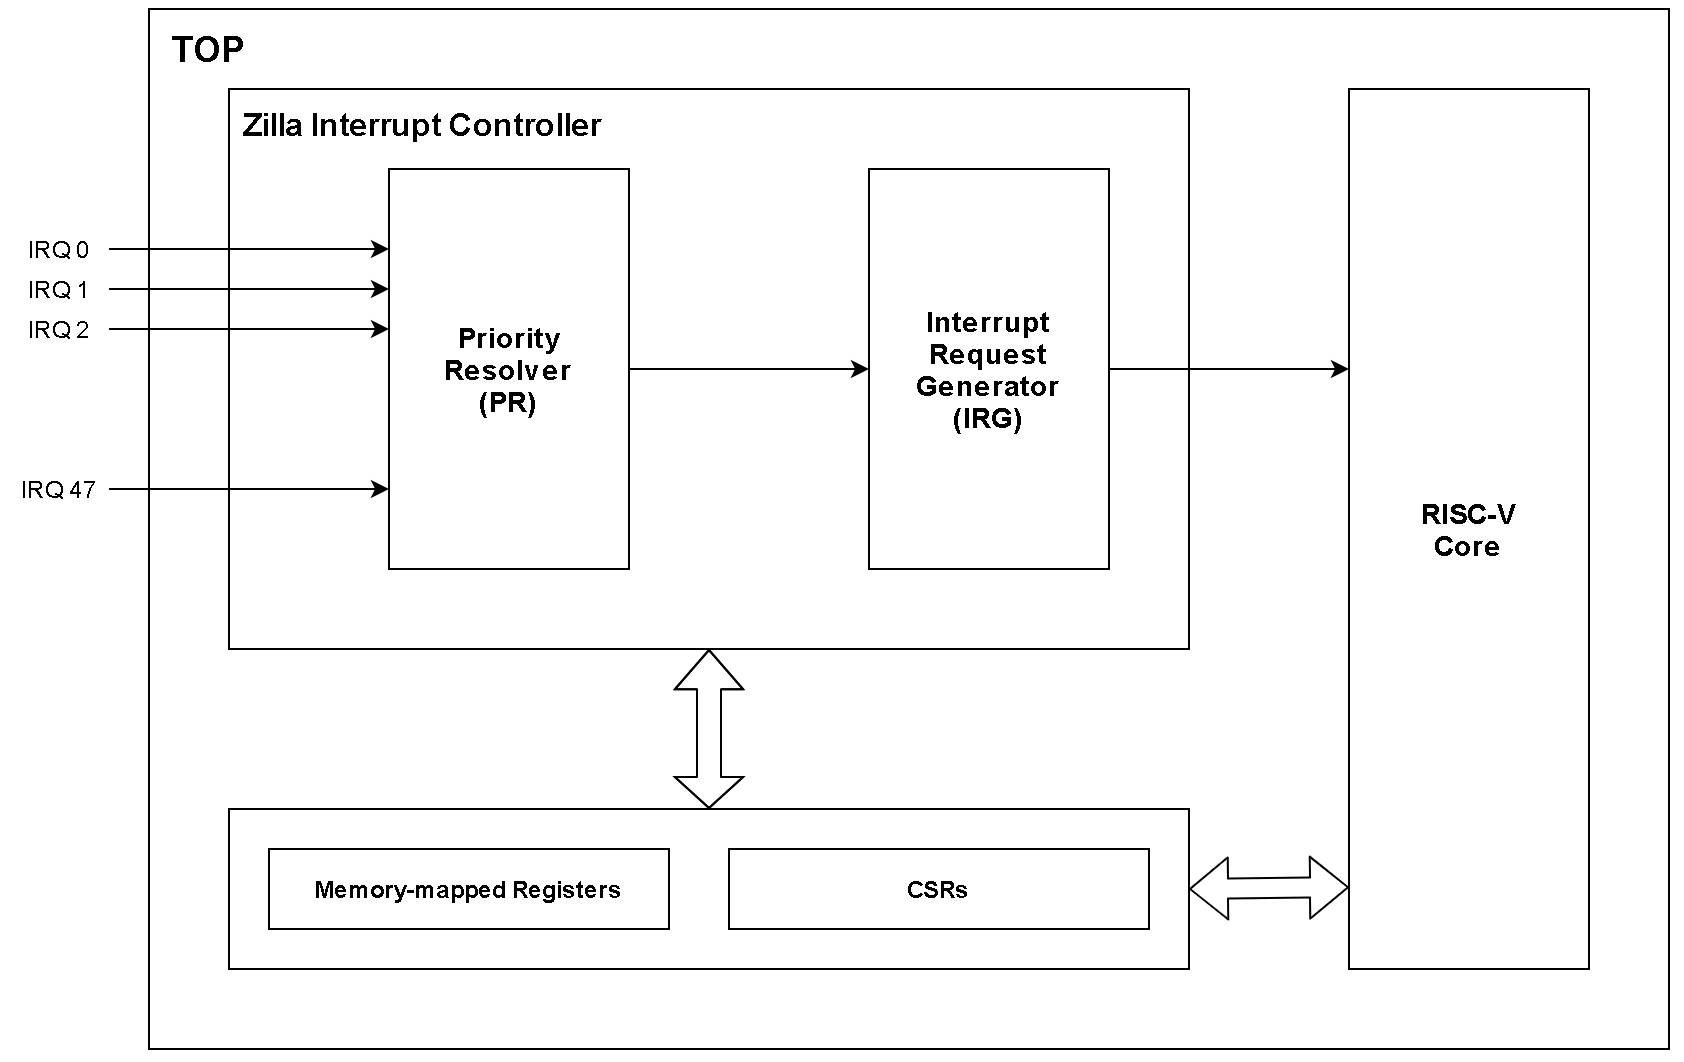
\includegraphics[width = 14cm]{images/ZIC.png}
    \vspace{1cm}
    \caption{\textbf{ZIC Partitioning}}
    \label{fig:zic_partitioning}
\end{figure}

\section{Priority Resolver}
\label{sec:priority-resolve}
The Priority Resolver block is responsible for  the following functionality.
\begin{enumerate}
    \item Provide an interface for all the external interrupts.
    \item Control the interrupt entry.
    \item Control the pending state of the interrupt.
    \item Assignment of level priority assignment for the pending interrupts and storing it in local buffers.
    \item Comparison of local buffers to obtain interrupt with highest level-priority value.
    \item Send the highest next pending interrupt to the Interrupt request generator.
\end{enumerate}

The Priority Resolver keeps track of new interrupts till the Interrupt Request Generator generates interrupt requests to the processor core. If any new interrupt is asserted from the source and has a higher level, the highest next pending register \texttt{zic\_nxtp\_int} is updated.

\subsection{Interrupt IDs}

\section{Interrupt Request Generator}
\label{sec:interrupt-request-generate}
The Interrupt Request Generator has the following functionality;
\begin{enumerate}
    \item Check for Sufficient Level-Priority.
    \item Update CSRs .
    \item Send a request to the core.
\end{enumerate}

This indicates the start of the interrupt service routine.

Once the processor completes the execution of the requested interrupt handler, it will write the corresponding ID into the end of the interrupt register \texttt{zi\_eoi}. Interrupt Request Generator detects this processor write and sends the new request for the next pending interrupt.


\chapter{Interrupt prioritization and handling overview}

Interrupt Handling and Prioritization Overview
This chapter describes the interrupt handling and prioritization in the ZIC. It contains the following sections:

\begin{itemize}
    \item \hyperref[sec:about-interrupt-priority-handling]{About interrupt prioritization and handling}
    \item \hyperref[sec:interrupt-levels-priorities]{Interrupt Levels and Priorities}
    \item \hyperref[sec:general-interrupt-handling]{General Interrupt Handling}
    \item \hyperref[sec:control-flow]{Control Flow}
    \item \hyperref[sec:isr]{Interrupt Service Routine}
    \item \hyperref[sec:interrupt-exit-flow]{Interrupt Exit Flow}
\end{itemize}
\newpage

\section{About interrupt prioritization and handling}
\label{sec:about-interrupt-priority-handling}

\section{Interrupt Levels and Priorities}
\label{sec:interrupt-levels-priorities}

Each supported interrupt has an interrupt ID and a programmable level priority value. Interrupt levels are used to determine preemption (for nesting interrupts). In contrast, Interrupt priorities do not affect preemption but are only used as a tie-breaker when there are multiple pending interrupts with the same interrupt level.

\subsection{Specifying Interrupt Level}

The 4-bit \texttt{zic\_cfg.nlbits} WARL field indicates how many upper bits in \linebreak \texttt{zic\_int\_ctl[i]} are assigned to encode the interrupt level. Valid values are 0-8.

Although the interrupt level is an 8-bit unsigned integer, the number of bits assigned or implemented can be fewer than 8. As described above, the number of bits assigned is specified in \texttt{cliccfg.nlbits}. The number of bits implemented can be derived from \texttt{zic\_cfg.nlbits} and a fixed parameter 
\linebreak \texttt{zic\_info.zic\_int\_ctl\_bits} (with a value between 0 to 8) which specifies bits implemented for both interrupts.

If the actual bits assigned or implemented are fewer than 8, then these bits are left-justified and appended with 1’s for the lower missing bits. 

For example, if the \texttt{nlbits > zic\_int\_ctl\_bits}, then the lower bits of the 8-bit, interrupt level are assumed to be all 1’s. Similarly, if \texttt{nlbits < 8}, then the lower bits of the 8-bit interrupt level are assumed to be all 1’s. Table \ref{tab:interrupt-level} shows how levels are encoded for these cases.

\vspace{1.25cm}
\begin{table}[H]
    \centering
    \caption{Encoding and Interrupt Levels}
    \label{tab:interrupt-level}
    \vspace{0.75cm}
    \begin{tabular}{|c|c|c|}
    \hline
        \textbf{No.} & & \\
        \textbf{of} & \textbf{Encoding\footnotemark} & \textbf{Interrupt Levels}\\
        \textbf{Bits} & & \\ \hline \hline
         0 & \texttt{........} & 255 \\ \hline
         1 & \texttt{l.......} & 127, 255 \\ \hline
         2 & \texttt{ll......} & 63, 127, 191, 255  \\ \hline
         3 & \texttt{lll.....} & 31, 63, 95, 127, 159, 191, 223, 255 \\ \hline
         4 & \texttt{llll....} & 15,31,47,63,79,95,111,127,143,159,175,191,207,223,239,255 \\ \hline
    \end{tabular}
\end{table}
\vspace{0.25cm}

\footnotetext{

"\texttt{l}" bits are available variable bits for level specification

"\texttt{.}" bits are non-existent bits for level encoding, assumed to be 1

If \texttt{nlbits}=0, then all interrupts are treated as level 255

}

Examples of \texttt{zic\_cfg} setting are shown in Table \ref{tab:zic-cfg-examples}.

\vspace{1.25cm}
\begin{table}[H]
    \centering
    \caption{ZIC Configuration Example for Interrupt Levels \& Priorities}
    \label{tab:zic-cfg-examples}
    \vspace{0.75cm}
    \begin{tabular}{|c|c|c|c|}
    \hline
        \textbf{\texttt{zic\_int\_ctl\_bits\footnotemark}} & \textbf{\texttt{nlbits}} & \textbf{\texttt{zic\_int\_ctl[i]}} & \textbf{Interrupt Levels}\\ \hline \hline
         0 & 2 & \texttt{........} & 255 \\ \hline
         1 & 2 & \texttt{l.......} & 127, 255 \\ \hline
         2 & 2 & \texttt{ll......} & 63, 127, 191, 255  \\ \hline
         3 & 3 & \texttt{lll.....} & 31, 63, 95, 127, 159, 191, 223, 255 \\ \hline
         4 & 1 & \texttt{lppp....} & 127, 255 \\ \hline
         6 & 3 & \texttt{lllppp..} & 31, 63, 95, 127, 159, 191, 223, 255 \\ \hline
    \end{tabular}
\end{table}
\vspace{0.25cm}

\footnotetext{

"\texttt{.}" bits are non-existent bits for level encoding, assumed to be 1

``\texttt{l}" bits are available variable bits for level specification

``\texttt{p}" bits are available variable bits for priority specification
}

\subsection{Specifying Interrupt Priority}

The least significant bits in \texttt{zic\_int\_ctl\_[i]} that are not configured to be part of the interrupt level, are part of interrupt priority, which are used to prioritize among interrupts pending and enabled at the same privilege mode and interrupt level. The highest-priority interrupt at a given privilege mode and interrupt level is taken first. 

In case there are multiple pending-and-enabled interrupts at the same highest priority, the highest-numbered interrupt is taken first. In other words, when privilege mode, level, and priority are all identical the highest-numbered interrupt wins in a tie.

Any implemented priority bits are treated as the most significant bits of an 8-bit unsigned integer with lower unimplemented bits set to 1. 

For example, with one priority bit \texttt{(p111\_1111)}, interrupts can be set to have priorities 127 or 255, and with two priority bits \texttt{(pp11\_1111)}, interrupts can be set to have priorities 63, 127, 191, or 255.

\section{General Interrupt Handling}
\label{sec:general-interrupt-handling}
The ZIC recognizes external interrupt requests and captures the interrupts that are supported. The ZIC maintains a state machine for each supported interrupt and all the operations are dependent on the interrupt state.

The ZIC interrupt handling sequence is

\begin{enumerate}
    \item The ZIC checks for the interrupt enable.
    \item The ZIC updates the pending status and assigns level priorities to the interrupts that are asserted.
    \item The ZIC compares level priorities of all pending interrupts and produces the highest next pending interrupt.
    \item The ZIC checks if the highest pending interrupt has sufficient priority.
    \item The ZIC sends an interrupt request to the core.
    \item The ZIC detects the processor acknowledging the interrupt request.
    \item The states and values are updated in the memory\-mapped registers and CSRs.
\end{enumerate}

In more detail, the steps are as follows

\begin{enumerate}
    \item The ZIC checks for the Local interrupt enable, which is controlled by the corresponding \texttt{zic\_int\_en[i]} register’s $0^{th}$ bit. Only enabled interrupts are considered by the Priority Resolver, else the corresponding interrupt will be ignored.
    \item If an enabled interrupt is asserted by the source, the status of that interrupt is changed to pending by setting the corresponding \texttt{zic\_int\_p[i]} register’s $0^{th}$ bit.
    \item Pending interrupts are assigned with level-priority values and are eligible for service by the processor core.
    \item If multiple enabled interrupts are asserted simultaneously, then level and priority comparison decide the highest next pending interrupt, which is eligible to be sent to the processor core.
    \item The level of highest pending interrupt is compared against the current level in the \texttt{mintstatus.mil}. After comparison, there are two possible outcomes
    \begin{enumerate}[label=(\alph*)]
        \item If the highest priority pending interrupt does not have sufficient priority, that Interrupt will be ignored.
        \item If the highest priority pending interrupt has sufficient priority, an interrupt request signal is sent to the processor.
    \end{enumerate}
    \item Meanwhile, the corresponding Interrupt ID is written into the \texttt{zic\_ack} acknowledge register.
    \item The processor acknowledges the interrupt request, by reading the interrupt ID from \texttt{zic\_ack} using a read-enable.
    \item The Interrupt Request Generator detects this read-enable and updates the current interrupt level CSR (\texttt{mintstatus.mil}).
\end{enumerate}

\section{Control Flow}
\label{sec:control-flow}

As soon as the interrupt is acknowledged by the core, the program control handles the entry procedure for an interrupt i into machine mode and is as follows,
\begin{enumerate}
    \item The cause of the interrupt is updated
    
    \texttt{mcause.interrupt = 1; mcause.exception\_code = i;}
    \item The previous interrupt enable is saved
    
    \texttt{mstatus.mpie = (See ISR stack.)}
    \item The previous privilege mode is saved
    
    \texttt{mstatus.mpp = M/S/U}
    \item The global Interrupts is disabled, interrupts remain disabled unless the ISR enables this.
    
    \texttt{mstatus.mie = 0}
    \item The \texttt{pc} (return address) is saved.
    
    \texttt{mepc = Interrupted pc.}
    \item The \texttt{pc} is updated.
    \begin{enumerate}
        \item Direct Mode i.e., \texttt{mtvec.mode == 0}, then 

        \texttt{pc = mtvec}
        \item Vectored Mode i.e.,  \texttt{mtvec.mode == 1}, then 
        
        \texttt{pc = mtvec+(i$\times$4)}
    \end{enumerate}
\end{enumerate}

Interrupts are enabled by the ISR to support interrupt nesting.

\section{Interrupt Service Routine}
\label{sec:isr}

\section{Interrupt Exit Flow}
\label{sec:interrupt-exit-flow}

The exit procedure for a machine interrupt when \texttt{mret} is executed is as follows,

\begin{enumerate}
    \item The Interrupt Enable is restored.
    
    \texttt{mstatus.mie = mstatus.mpie}
    \item The Privilege mode is restored.
    
    \texttt{M/S/U = mstatus.mpp}
    \item The \texttt{pc} is restored.
    
    \texttt{pc = mepc}
\end{enumerate}



\chapter{Programmers' Model}
This chapter describes the ZIC Memory-mapped registers and CSRs. It contains the following sections:
\begin{itemize}
    \item \hyperref[sec:about-programmers-model]{About the Programmers' Model}
    \item \hyperref[sec:zic-mem-map-register-description]{ZIC memory-mapped register description}
    \item \hyperref[sec:zic-csr-description]{ZIC CSRs description}
\end{itemize}
\newpage

\section{About the Programmers' Model}
\label{sec:about-programmers-model}
The programmers’ model provides the software interface to the ZIC. This chapter describes the programmers’ model for the ZIC Priority Resolver and Interrupt Request Generator that operates using ZIC memory-mapped registers and CSRs.

The following sections describe the programmers’ model:
\begin{itemize}
    \item \hyperref[subsec:zic-register-mem-map]{ZIC register memory-map}
    \item \hyperref[subsec:zic-csrs-mem-map]{ZIC CSRs memory-map}
\end{itemize}

\subsection{ZIC registers memory-map}
\label{subsec:zic-register-mem-map}
Zilla core has ZIC registers that are accessed by a separate address region. ZIC registers are accessible by the M-mode software running on the Zilla core. The base address of ZIC memory-mapped registers is specified by \texttt{mzicbase} machine CSR.

The ZIC supports up to 48 total interrupt inputs. Table \ref{tab:zic-reg-memory-map} has a list of memory-mapped registers for ZIC.

\vspace{1.25cm}
\begin{table}[H]
    \centering
    \caption{ZIC register memory-map}
    \label{tab:zic-reg-memory-map}
    \vspace{0.75cm}
    \begin{tabular}{l l l l}
    \hline 
        \textbf{Offset} & \textbf{Name} & \textbf{Type} & \textbf{Description}  \\ \hline \hline
        \texttt{0x0000} & \texttt{\hyperref[subsec:zic-cfg]{zic\_cfg}} & R & ZIC Configuration Register \\ \hline
        \texttt{0x0004} & \texttt{\hyperref[subsec:zic-info]{zic\_info}} & R & ZIC Information Register \\ \hline
        \texttt{0x0800} & \texttt{\hyperref[subsec:zic-nxtp-int]{zic\_nxtp\_int}} & R & ZIC Next-Pending Interrupt Register \\ \hline
        \texttt{0x0804} & \texttt{\hyperref[subsec:zic-ack]{zic\_ack}} & R & ZIC Acknowledgement Register \\ \hline
         \texttt{0x0808} & \texttt{\hyperref[subsec:zic-eoi]{zic\_eoi}} & R & ZIC End-of-Interrupt Register \\ \hline 
         & & &  \\ \hline
         \texttt{0x1000} & \texttt{\hyperref[subsec:zic-int-p]{zic\_int\_p\_[0]}} & RW & ZIC Interrupt Pending Register [0] \\ \hline
         \texttt{0x1001} & \texttt{\hyperref[subsec:zic-int-en]{zic\_int\_en\_[0]}} & RW & ZIC Interrupt Enable Register [0]\\ \hline
         \texttt{0x1002} & \texttt{\hyperref[subsec:zic-int-attr]{zic\_int\_attr\_[0]}} & R & ZIC Interrupt Attribute Register [0] \\ \hline
         \texttt{0x1003} & \texttt{\hyperref[subsec:zic-int-ctl]{zic\_int\_ctl\_[0]}} & RW & ZIC Interrupt Control Register [0] \\ \hline
         : & : & : & : \\ \hline
         \texttt{0x10BC} & \texttt{\hyperref[subsec:zic-int-p]{zic\_int\_p\_[47]}} & RW & ZIC Interrupt Pending Register [47]\\ \hline
         \texttt{0x10BD} & \texttt{\hyperref[subsec:zic-int-en]{zic\_int\_en\_[47]}} & RW & ZIC Interrupt Enable Register [47] \\ \hline
         \texttt{0x10BE} & \texttt{\hyperref[subsec:zic-int-attr]{zic\_int\_attr\_[47]}} & R & ZIC Interrupt Attribute Register [47] \\ \hline
         \texttt{0x10BF} & \texttt{\hyperref[subsec:zic-int-ctl]{zic\_int\_ctl\_[47]}} & RW & ZIC Interrupt Control Register [47] \\ \hline
        \end{tabular}
\end{table}

\subsection{ZIC CSRs memory-map}
\label{subsec:zic-csrs-mem-map}
Zilla core has Machine CSRs, some of which are dedicated for interrupt-handling. These CSRs are accessible by ZIC and also by CSR op-codes.

The interrupt-handling CSRs are listed is Table \ref{tab:zic-csr-memory-map}. The changes to existing CSRs and addition of new CSRs for ZIC mode operation are explained in the ZIC CSRs description.

\vspace{1.25cm}
\begin{table}[H]
    \centering
    \caption{ZIC CSRs memory-map}
    \label{tab:zic-csr-memory-map}
    \vspace{0.75cm}
    \begin{tabular}{l l l l}
    \hline 
        \textbf{Address} & \textbf{Name} & \textbf{Type} & \textbf{Description} \\ \hline \hline
        \texttt{} & \texttt{\hyperref[subsec:mstatus]{mstatus}} & RW & Machine Status Register \\ \hline 
        \texttt{} & \texttt{\hyperref[subsec:mtvec]{mtvec}} & RW & Machine Trap Vector Register \\ \hline
        \texttt{} & \texttt{\hyperref[subsec:mtvt]{mtvt}} & RW & Machine Trap Vector Table Register \\ \hline
        \texttt{} & \texttt{\hyperref[subsec:mscratch]{mscratch}} & RW & Machine Scratch Register \\ \hline
        \texttt{} & \texttt{\hyperref[subsec:mepc]{mepc}} & RW & Machine Exception \texttt{pc} Register \\ \hline
        \texttt{} & \texttt{\hyperref[subsec:mcause]{mcause}} & RW & Machine Cause Register \\ \hline
        \texttt{} & \texttt{\hyperref[subsec:mintstatus]{mintstatus}} & RW & Machine Interrupt Status Register \\ \hline
        \texttt{} & \texttt{\hyperref[subsec:mzicbase]{mzicbase}} & RW & Machine ZIC Base Register \\ \hline
        \end{tabular}
\end{table}

\section{ZIC memory-mapped register description}
\label{sec:zic-mem-map-register-description}

\subsection{ZIC Configuration Register, \texttt{zic\_cfg}}
\label{subsec:zic-cfg}

ZIC has a single memory-mapped 8-bit global configuration register, that defines how many privilege modes are supported, how the \texttt{\hyperref[subsec:zic-int-ctl]{zic\_int\_ctl\_[i]}} registers are subdivided into level and priority fields, and whether selective hardware vectoring is supported.

\vspace{0.5cm}
\begin{figure}[H]
    \centering
    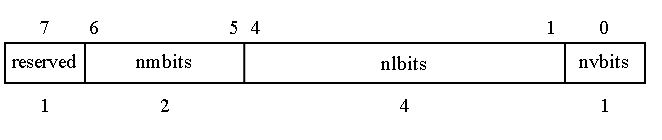
\includegraphics[width = 9cm]{images/zic_cfg.png}
    \label{fig:zic_cfg}
\end{figure}
\vspace{0.25cm}

\vspace{0.5cm}
\begin{table}[H]
    \label{tab:zic_cfg}
        \centering
        \begin{tabular}{l l p{8cm} c c}
         \hline 
         \textbf{Bits} & \textbf{Name} & \textbf{Description} & \textbf{Access} & \textbf{Preset}\\ \hline \hline
         [7] & reserved & - & - & 0 \\ \hline
         [6:5] & \texttt{nmbits} & Specifies how many bits are physically implemented in \texttt{zic\_int\_attr\_[i].mode} to represent an input i's privilege mode.
         
         0: M-mode Only
         
         1: M/U Modes
         
         2: M/U/S Modes
         
         3: Reserved & R & 0 \\ \hline
         [4:1] & \texttt{nlbits} & Indicates how many upper bits in \texttt{zic\_int\_ctl\_[i]} are assigned to encode the interrupt levels. 
         
         Valid values are 0-8. & R & 3\\ \hline
         [0] & \texttt{nvbits} & Specifies whether the selective interrupt hardware vectoring feature is implemented or not.
         
         0: selective interrupt hardware vectoring is not implemented.
         
         1: selective interrupt hardware vectoring is implemented. & R & 0\\ \hline
         \end{tabular}
\end{table}

\subsection{ZIC Information Register, \texttt{zic\_info}}
\label{subsec:zic-info}

This is an 8-bit register that holds information such as number of triggers implemented, number of interrupts supported, architecture and implementation version which are useful for debugging.

\vspace{0.5cm}
\begin{figure}[H]
    \centering
    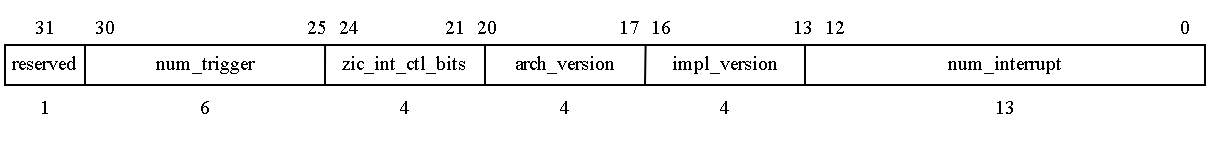
\includegraphics[width = 15.25cm]{images/zic_info.png}
    \label{fig:zic_cfg}
\end{figure}
\vspace{0.25cm}

\vspace{0.5cm}
\begin{table}[H]
    \label{tab:zic_info}
        \centering
        \begin{tabular}{l l p{6cm} c c}
         \hline 
         \textbf{Bits} & \textbf{Name} & \textbf{Description} & \textbf{Access} & \textbf{Preset}\\ \hline \hline
         [31] & reserved & - & - & 0 \\ \hline
         [30:25] & \texttt{num\_trigger} & Specifies the number of maximum interrupt triggers supported in this implementation.
         
         Valid values are 0-32. & R & 0\\ \hline
         [24:21] & \texttt{zic\_int\_ctl\_bits\footnotemark} & Specifies how many hardware bits are implemented in the \texttt{zic\_int\_ctl} registers. 

         Valid values are 0-8. & R & 6\\ \hline
         [20:17] & \texttt{arch\_version} & Specifies Architecture Version. & R & 0\\ \hline
         [16:13] & \texttt{impl\_version} & Specifies Implementation Version. & R & 0 \\ \hline
         [12:10] & \texttt{num\_interrupts} & Specifies the actual number of maximum interrupt inputs supported in this implementation & R & 47 \\ \hline
         \end{tabular}
\end{table}

\footnotetext{The implemented bits are kept left-justified in the most significant bits of each 8-bit \texttt{zic\_int\_ctl\_[i]} register, with the lower unimplemented bits treated as hardwired to 1.}

\subsection{ZIC Next-Pending Interrupt Register, \texttt{zic\_nxtp\_int}}
\label{subsec:zic-nxtp-int}
This is an 8-bit register that holds the level of highest pending interrupt.

\vspace{0.5cm}
\begin{figure}[H]
    \centering
    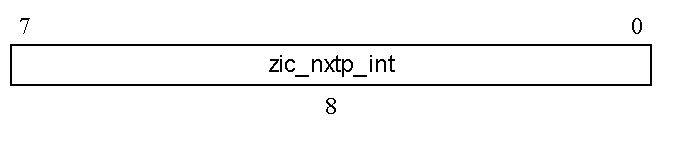
\includegraphics[width = 9cm]{images/zic_nxtp_int.png}
    \label{fig:zic_nxtp_int}
\end{figure}
\vspace{0.25cm}

\vspace{0.5cm}
\begin{table}[H]
    \label{tab:zic_nxtp_int}
        \centering
        \begin{tabular}{l l p{7cm} c c}
         \hline 
         \textbf{Bits} & \textbf{Name} & \textbf{Description} & \textbf{Access} & \textbf{Preset}\\ \hline \hline
         [7:0] & \texttt{zic\_nxtp\_int} & This register will be written with the highest level of pending interrupt after priority resolution. & RW & 0\\ \hline
        \end{tabular}
\end{table}
\vspace{0.5cm}

Priority Resolver performs a comparison of all the pending interrupts by comparing the local buffers to check which interrupt has the highest level-priority value. At the end of the comparison, the level-priority value of that interrupt is written to this register.

Interrupt Request Generator reads this register and compares it with the current interrupt level form \texttt{\hyperref[subsec:mintstatus]{mintstatus}} and decides whether the highest pending interrupt has sufficient priority.

\subsection{ZIC Acknowledgement Register, \texttt{zic\_ack}}
\label{subsec:zic-ack}
This is an 8-bit register that holds the ID value of the requested interrupt, before the acknowledgment from the processor.

\vspace{0.5cm}
\begin{figure}[H]
    \centering
    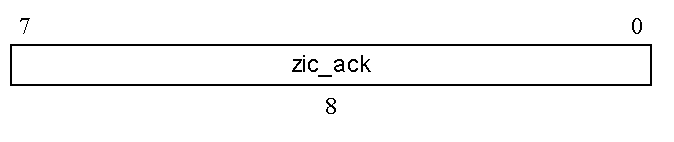
\includegraphics[width = 9cm]{images/zic_ack.png}
    \label{fig:zic_ack}
\end{figure}
\vspace{0.25cm}

\vspace{0.5cm}
\begin{table}[H]
    \label{tab:zic_ack}
        \centering
        \begin{tabular}{l l p{8cm} c c}
         \hline 
         \textbf{Bits} & \textbf{Name} & \textbf{Description} & \textbf{Access} & \textbf{Preset}\\ \hline \hline
         [7:0] & \texttt{zic\_ack} & This register will be read by the processor to serve the interrupt. & RW & 0\\ \hline
        \end{tabular}
\end{table}
\vspace{0.5cm}

 When the processor reads this register, Interrupt Request Generator recognizes this read, clears the pending bit in \texttt{zic\_int\_p\_[i]}, and writes the level-priority value into \texttt{mintstatus} CSR.

\subsection{ZIC End-of-Interrupt Register, \texttt{zic\_eoi}}
\label{subsec:zic-eoi}
This is an 8-bit register that holds the ID value of interrupt currently being served.

\vspace{0.5cm}
\begin{figure}[H]
    \centering
    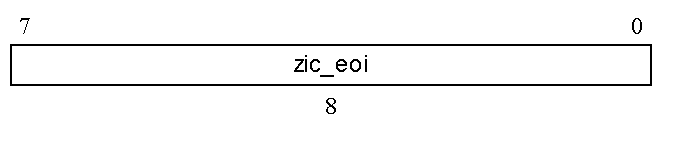
\includegraphics[width = 9cm]{images/zic_eoi.png}
    \label{fig:zic_eoi}
\end{figure}
\vspace{0.25cm}

\vspace{0.5cm}
\begin{table}[H]
    \label{tab:zic_eoi}
        \centering
        \begin{tabular}{l l p{8cm} c c}
         \hline 
         \textbf{Bits} & \textbf{Name} & \textbf{Description} & \textbf{Access} & \textbf{Preset}\\ \hline \hline
         [7:0] & \texttt{zic\_eoi} & The processor writes the ID of the interrupt into this register once it completes executing the ISR. & RW & 0\\ \hline
        \end{tabular}
\end{table}
\vspace{0.5cm}

\subsection{ZIC Interrupt Pending Registers, \texttt{zic\_int\_p\_[i]}}
\label{subsec:zic-int-p}
Every interrupt supported by the platform has a dedicated interrupt pending register and occupies one byte in the memory map for ease of access. The pending bit is located in bit 0 of the byte.

\vspace{0.5cm}
\begin{figure}[H]
    \centering
    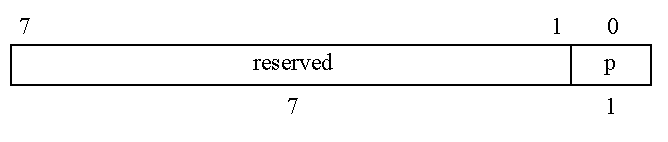
\includegraphics[width = 9cm]{images/zic_int_p.png}
    \label{fig:zic_int_p}
\end{figure}
\vspace{0.25cm}

\vspace{0.5cm}
\begin{table}[H]
    \label{tab:zic_int_p}
        \centering
        \begin{tabular}{l l p{8cm} c c}
         \hline 
         \textbf{Bits} & \textbf{Name} & \textbf{Description} & \textbf{Access} & \textbf{Preset} \\ \hline \hline
         [7:1] & reserved & - & - & 0 \\ \hline
         [0] & p & 0: Interrupt is requested from the source
         
         1: Interrupt is de-asserted from the source
 & RW & 0\\ \hline
        \end{tabular}
\end{table}
\vspace{0.5cm}

If the interrupt line is enabled globally and is asserted from the source, the Priority Resolver sets the corresponding interrupt pending register bit.

Priority Resolver will clear this bit when the End of Interrupt signal is detected.

\subsection{ZIC Interrupt Enable Registers, \texttt{zic\_int\_en\_[i]}}
\label{subsec:zic-int-en}

Every interrupt supported by the platform has a dedicated interrupt enable register and occupies one byte in the memory map for ease of access. This enable bit is located in bit 0 of the byte.

\vspace{0.5cm}
\begin{figure}[H]
    \centering
    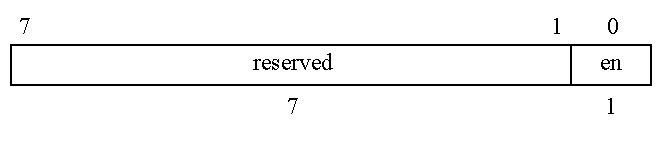
\includegraphics[width = 9cm]{images/zic_int_en.png}
    \label{fig:zic_int_en}
\end{figure}
\vspace{0.25cm}

\vspace{0.5cm}
\begin{table}[H]
    \label{tab:zic_int_en}
        \centering
        \begin{tabular}{l l p{8cm} c c}
         \hline 
         \textbf{Bits} & \textbf{Name} & \textbf{Description} & \textbf{Access} & \textbf{Preset}\\ \hline \hline
         [7:1] & reserved & - & - & 0 \\ \hline
         [0] & en & 0: Interrupt is disabled
         
         1: Interrupt is enabled & RW & 0\\ \hline
        \end{tabular}
\end{table}
\vspace{0.5cm}

\subsection{ZIC Interrupt Attribute Registers, \texttt{zic\_int\_attr\_[i]}}
\label{subsec:zic-int-attr}

This is an 8-bit register that specify various attributes such as privilege mode, trigger type and hardware vectoring for each interrupt.

\vspace{0.5cm}
\begin{figure}[H]
    \centering
    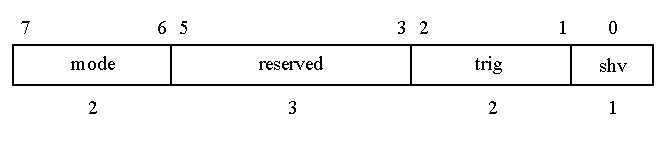
\includegraphics[width = 9cm]{images/zic_int_attr.png}
    \label{fig:zic_int_attr}
\end{figure}
\vspace{0.5cm}

\vspace{0.5cm}
\begin{table}[H]
    \label{tab:zic_int_attr}
        \centering
        \begin{tabular}{l l p{8cm} c c}
         \hline 
         \textbf{Bits} & \textbf{Name} & \textbf{Description} & \textbf{Access} & \textbf{Preset}\\ \hline \hline
         [7:6] & mode & Specifies which privilege mode this interrupt operates in
         
         11: machine mode 
         
         01: supervisor mode
         
         00: user mode & R & 3 \\ \hline
         [5:3] & reserved & - & - & 0 \\ \hline
         [2:1] & trig & Specifies the trigger type and polarity for each interrupt
         
         00: Positive level-triggered
         
         01: Positive edge-triggered
         
         10: Negative level-triggered
         
         11: Negative edge-triggered & R & \\ \hline
         [0] & shv & Selective Hardware Vectoring & R & \\ \hline
        \end{tabular}
\end{table}
\vspace{0.5cm}

\subsection{ZIC Interrupt Control Registers, \texttt{zic\_int\_ctl\_[i]}}
\label{subsec:zic-int-ctl}

This is an 8-bit memory-mapped register to control the interrupt pre-emption (nesting) using levels and priorities. The number of bits implemented in this register is specified by a fixed parameter \texttt{zic\_int\_ctl\_bits} (in \texttt{zic\_info}), which has a value between 0 to 8. 

The implemented bits are kept left-justified in the most significant bits of each 8-bit \texttt{zic\_int\_ctl\_[i]} register, with the lower unimplemented bits treated as hardwired to 1.

These control bits are interpreted as level and priority according to the setting in the ZIC
Configuration register (\texttt{zic\_cfg.nlbits}).

\vspace{0.5cm}
\begin{figure}[H]
    \centering
    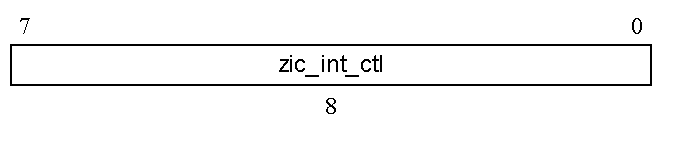
\includegraphics[width = 9cm]{images/zic_int_ctl.png}
    \label{fig:zic_int_ctl}
\end{figure}
\vspace{0.25cm}

\vspace{0.5cm}
\begin{table}[H]
    \label{tab:zic_int_ctl}
        \centering
        \begin{tabular}{l l p{8cm} c c}
         \hline 
         \textbf{Bits} & \textbf{Name} & \textbf{Description} & \textbf{Access} & \textbf{Preset}\\ \hline \hline
         [7:0] & \texttt{zic\_int\_ctl} & Specifies the Level and Priority of the interrupt & RW & 0\\ \hline
        \end{tabular}
\end{table}
\vspace{0.5cm}

When an interrupt is enabled and the corresponding pending bit is set, Priority Resolver loads the level-priority value into a local buffers, holding the pending bit and level-priority value.

\section{ZIC CSRs Description}
\label{sec:zic-csr-description}

\subsection{Machine Status Register, \texttt{mstatus}}
\label{subsec:mstatus}

This is a 64-bit CSR that keeps track of and controls the hart's current operating state.

\texttt{mie} is hardwired to zero in ZIC mode, replaced by separate memory-mapped interrupt enable registers (\texttt{zic\_int\_en\_[i]}).

\texttt{mip} is hardwired to zero in ZIC mode, replaced by separate memory-mapped interrupt pending registers (\texttt{zic\_int\_p\_[i]}).

Writes to \texttt{mie/mip} will be ignored and will not trap (i.e., no access faults). 

\subsection{Machine Trap Vector Register, \texttt{mtvec}}
\label{subsec:mtvec}

This is a 64-bit CSR that holds trap vector configuration, consisting of a vector base address (BASE) and a vector mode (MODE).

\vspace{0.5cm}
\begin{figure}[H]
    \centering
    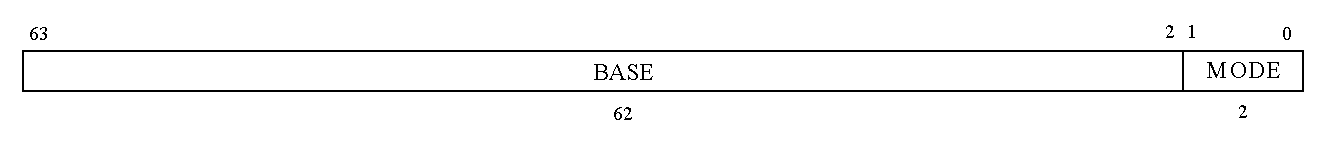
\includegraphics[width = 15.25cm]{images/csr_mtvec.png}
    \label{fig:csr_mtvec}
\end{figure}
\vspace{0.25cm}

\vspace{0.5cm}
\begin{table}[H]
    \label{tab:csr_mtvec}
        \centering
        \begin{tabular}{l l p{8cm} c c}
         \hline 
         \textbf{Bits} & \textbf{Name} & \textbf{Description} & \textbf{Access} & \textbf{Preset}\\ \hline \hline
         [63:2] & BASE & Specifies the base address & WARL & 0 \\ \hline
         [1:0] & MODE & Specifies the mode of operation
         
         0: Direct - All exceptions are in Direct mode 
         
         \hspace{1cm} \texttt{pc} = BASE.
         
         1: Vectored - All asynchronous interrupts are in Vectored mode
         
         \hspace{1cm} \texttt{pc} = BASE + (4 $\times$ cause).
         
         $\geq$ 2: Reserved & WARL & 0\\ \hline
        \end{tabular}
\end{table}
\vspace{0.5cm}

\subsection{Machine Trap Vector Table Register, \texttt{mtvt}}
\label{subsec:mtvt}

This is a 64-bit CSR that holds the base address of the trap vector table.

\vspace{0.5cm}
\begin{figure}[H]
    \centering
    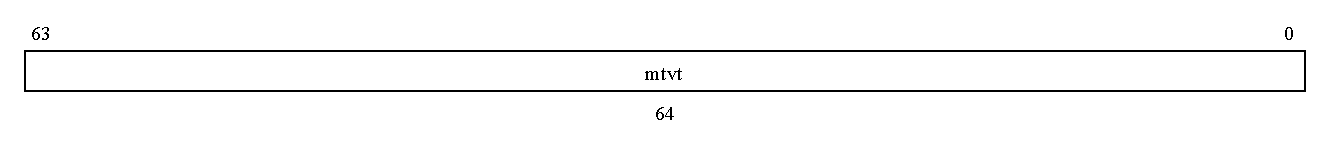
\includegraphics[width = 15.25cm]{images/csr_mtvt.png}
    \label{fig:csr_mtvt}
\end{figure}
\vspace{0.25cm}

It is aligned on a 64-byte or greater power-of-two boundary. 

The actual alignment can be determined by writing ones to the low-order bits then reading them back. Values other than 0 in the low 6 bits of \texttt{xtvt} are reserved.

\subsection{Machine Scratch Register, \texttt{mscratch}}
\label{subsec:mscratch}

This is a 64-bit CSR dedicated for use by machine mode.

\vspace{0.5cm}
\begin{figure}[H]
    \centering
    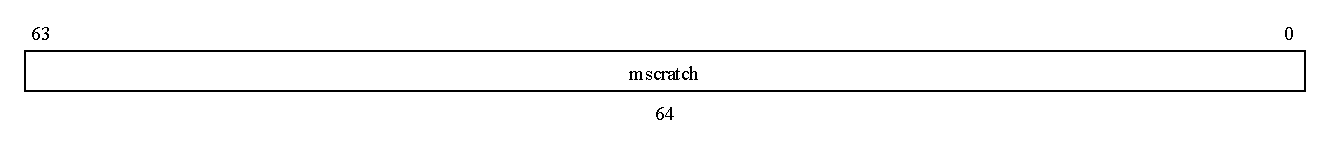
\includegraphics[width = 15.25cm]{images/csr_mscratch.png}
    \label{fig:csr_mscratch}
\end{figure}
\vspace{0.25cm}

Typically, it is used to hold a pointer to a machine-mode hart-local context space and swapped with a user register upon entry to an M-mode trap handler.

\subsection{Machine Exception \texttt{pc} Register, \texttt{mepc}}
\label{subsec:mepc}

This is a 64-bit register that stores the \texttt{pc} value when normal execution is interrupted.

\vspace{0.5cm}
\begin{figure}[H]
    \centering
    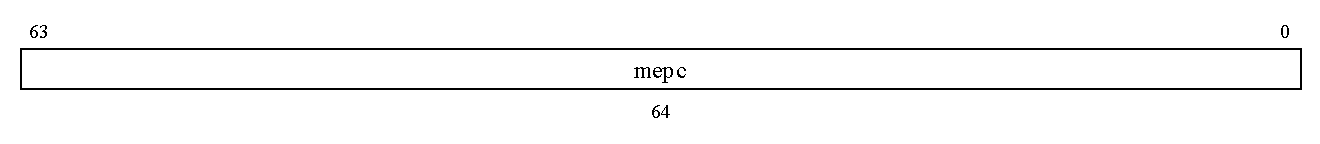
\includegraphics[width = 15.25cm]{images/csr_mepc.png}
    \label{fig:csr_mepc}
\end{figure}
\vspace{0.25cm}

\subsection{Machine Cause Register, \texttt{mcause}}
\label{subsec:mcause}

This is a 64-bit CSR that holds the information regarding cause of trap and additional book-keeping like previous interrupt status. When a trap is taken into M-mode, \texttt{mcause} is written with a code indicating the event that caused the trap.

Otherwise, mcause is never written by the implementation, though it may be explicitly written by software.

\vspace{0.5cm}
\begin{figure}[H]
    \centering
    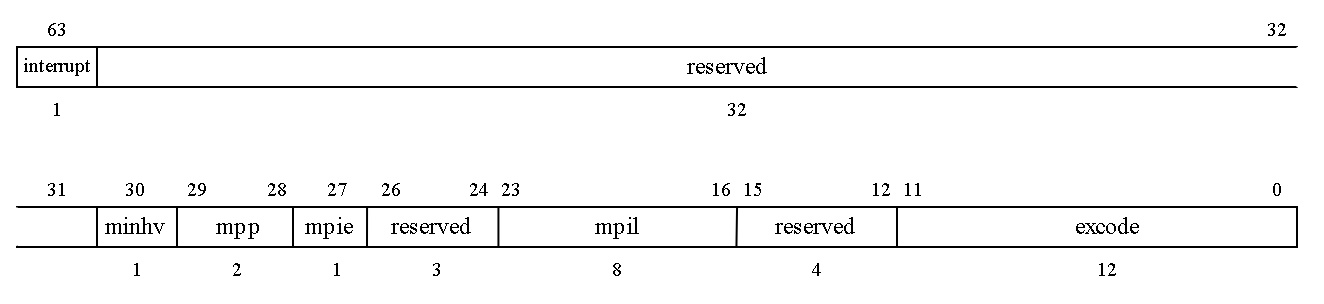
\includegraphics[width = 15.25cm]{images/csr_mcause.png}
    \label{fig:csr_mcause}
\end{figure}
\vspace{0.25cm}

\vspace{0.5cm}
\begin{table}[H]
    \label{tab:csr_mcause}
        \centering
        \begin{tabular}{l l p{8cm} c c}
         \hline 
         \textbf{Bits} & \textbf{Name} & \textbf{Description} & \textbf{Access} & \textbf{Preset} \\ \hline \hline
         [63] & interrupt & Specifies the type of trap.
         
         0: Exception
         
         1: Interrupt & RW & 0\\ \hline
         [62:31] & reserved & - & - & 0\\ \hline
         [30] & minhv & Specifies the status of the Hardware Vectoring
         
         0: End of successful hardware vectoring
         
         1: Start of hardware vectoring & R & 0\\ \hline
         [29:28] & mpp & Previous privilege mode
         
         (same as mstatus.mpp) & R & 3\\ \hline
         [27] & mpie & Previous Interrupt Enable & R & 0\\ \hline
         [26:24] & reserved & - & - & 0\\ \hline
         [23:16] & mpil & Previous interrupt level & R \\ \hline
         [15:12] & reserved & - & - & 0\\ \hline
         [11:0] & excode & Exception/interrupt code & WARL & 0\\ \hline
        \end{tabular}
\end{table}
\vspace{0.5cm}

\subsection{Machine Interrupt Status, \texttt{mintstatus}}
\label{subsec:mintstatus}

This is a 64-bit CSR that holds the active interrupt level for machine privilege mode. The primary reason to expose these fields is to support debugging.

\vspace{0.5cm}
\begin{figure}[H]
    \centering
    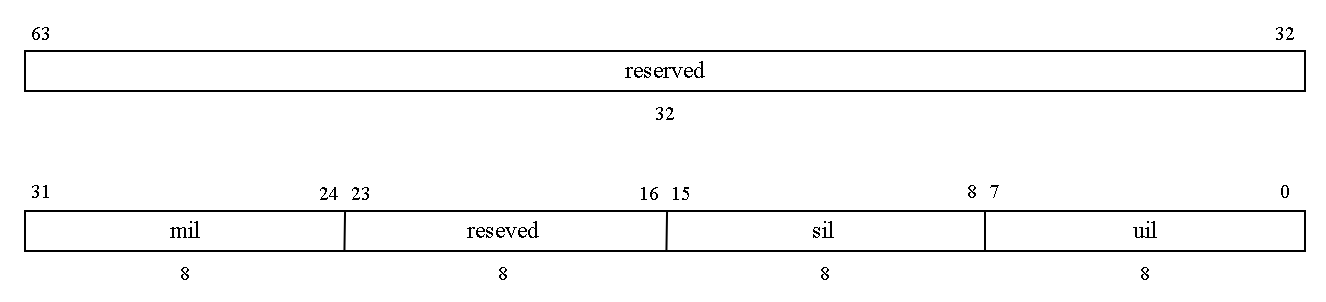
\includegraphics[width = 15.25cm]{images/csr_mintstatus.png}
    \label{fig:csr_mintstatus}
\end{figure}
\vspace{0.25cm}

\vspace{0.5cm}
\begin{table}[H]
    \label{tab:csr_mintstatus}
        \centering
        \begin{tabular}{l l p{8cm} c c}
         \hline 
         \textbf{Bits} & \textbf{Name} & \textbf{Description} & \textbf{Access} & \textbf{Preset}\\ \hline \hline
         [63:32] & reserved & - & - & 0\\ \hline
         [31:24] & mil & Specifies Machine-mode active Interrupt Level & R & 0\\ \hline
         [23:16] & reserved & - & - & 0\\ \hline
         [15:8] & sil & Specifies Supervisor-mode active Interrupt Level
         
         This field is harwired to 0. & R & 0\\ \hline
         [7:0] & uil & Specifies User-mode active Interrupt Level
         
         This field is harwired to 0. & R & 0\\ \hline
        \end{tabular}
\end{table}
\vspace{0.5cm}

Interrupt Request Generator reads \texttt{mil} value and compares it with the \linebreak \texttt{zic\_nxtp\_int} value to decide whether the next pending interrupt has sufficient level priority. 

If the new interrupt has sufficient priority, then the Interrupt Request Generator generates interrupt requests to the core processor and writes corresponding Interrupt ID into the \texttt{zic\_ack} register.


\subsection{Machine ZIC Base Register, \texttt{mzicbase}}
\label{subsec:mzicbase}

This is a 64 - bit  CSR that stores the base address of the memory-mapped ZIC registers.

\vspace{0.5cm}
\begin{figure}[H]
    \centering
    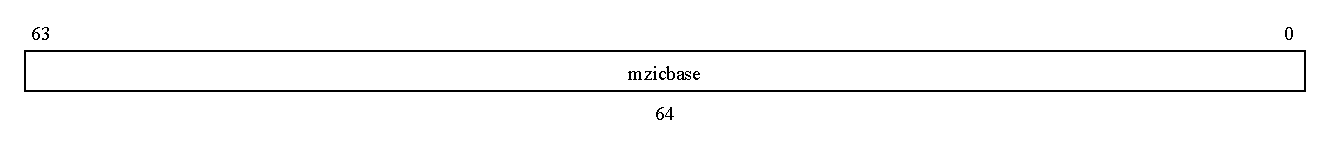
\includegraphics[width = 15.25cm]{images/csr_mzicbase.png}
    \label{fig:csr_mzicbase}
\end{figure}
\vspace{0.25cm}

\vspace{0.5cm}
\begin{table}[H]
    \label{tab:csr_mzicbase}
        \centering
        \begin{tabular}{l l p{8cm} c c}
         \hline 
         \textbf{Bits} & \textbf{Name} & \textbf{Description} & \textbf{Access} & \textbf{Preset}\\ \hline \hline
         [63:0] & mzicbase & Base address for ZIC memory-mapped register & R & 0\\ \hline
        \end{tabular}
\end{table}
\vspace{0.5cm}


\addcontentsline{toc}{chapter}{References}
\bibliographystyle{ieeetr}
\bibliography{References}
\nocite{*}

\end{document}
